\textbf{Cas d'utilisation:} Payer avec du liquide

\textbf{Acteur primaire:} Conducteur
%(initiateur) poste surveillance

%\textbf{Acteur support:}

\textbf{Pré-condition: } la borne affiche le montant
 
%\textbf{Post-condition: } 

\textbf{Scénario primaire: } \\
    \textbf{1.} La borne reçoit de l’argent liquide du conducteur.\\
    \textbf{2.} La borne enclenche la détection de fausse pièce. Valide les pieces\\
    \textbf{3.} Le borne regarde le montant.Le conducteur a donné le montant exact\\
    \textbf{4.}La borne accepte le paiement.

\textbf{Variantes:}\\
    \textbf{2a.} valide pas les pieces - rend pieces invalides.\\
    \textbf{3a.} Le conducteur donne un montant plus grand que celui de la borne il rend la différence entre la somme introduite et le montant demandé. \\
    \textbf{3b.} Le conducteur donne un montant moins que celui de la borne. Se met en attente.\\
    \textbf{4a.} Le borne ne accepte pas le paiement (car un problème technique au car le conducteur il n'y a pas comment payer). Appelle le technicien. \\
    \textbf{3a1.} la borne n’a plus de monnaie, elle émet un signal vers un technicien.\\

%2. a 1) la borne n’a plus de monnaie, elle émet un signal vers un technicien

%\textbf{Décomposition des cas d'utilisation:} 
%\begin{figure}[h]
 %   \centering
  %  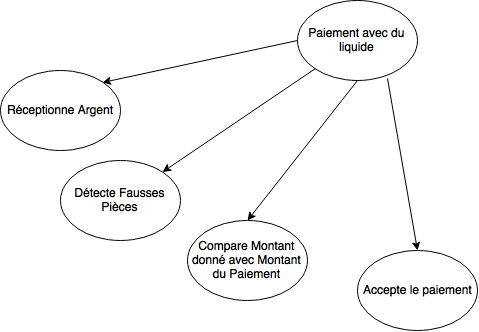
\includegraphics[scale=0.48]{02_Desenvolvimento/TD2/images/PaiementLiquide.png}
   % \caption{Décomposition des cas d'utilisation: Payer avec du liquide}
%\end{figure}
